\documentclass[]{article}

\usepackage{amsmath}
\usepackage{float}
\usepackage{circuitikz}
\usepackage{tikz}
\usepackage{pgfplots}

\usetikzlibrary{shapes.misc}

\tikzset{cross/.style={cross out, draw=black, minimum size=2*(#1-\pgflinewidth), inner sep=0pt, outer sep=0pt},
%default radius will be 1pt. 
cross/.default={10pt}}

\author{Abdelsalam ElTamawy 900170376\\Emman\\Nada Badawy 900171975}
\date{\today}
\title{CSCE 3304 - Digital Design 2\\Project 1\\A small standard cell library\\}

\begin{document}
	
\begin{titlepage}
	\maketitle
\end{titlepage}

\tableofcontents

\pagebreak

\section{Introduction}

\section{Inverter}
\subsection{Schematic}

\begin{figure}[H]
	\centering
	\begin{circuitikz}
		\draw
		(0,0) node[nmos] (na) {}
		(na.G) node[left] {$in$}
		(na.D) node[pmos,anchor=D] (pa) {}
		(pa.G) node[left] {$in$}
		(na.D) -- ++(1,0) node[right] {$f$}
		(na.S) node[ground] {}
		(pa.S) node[vdd] {$3.3$V}
		;
	\end{circuitikz}
	\caption{}
	\label{}
\end{figure}

\subsection{Stick diagram}
\subsection{Schematic}
\section{Tri-state Inverter}
\subsection{Schematic}
	\begin{figure}[H]
	\centering
	\begin{circuitikz}
		\draw
		(0,0) node[nmos] (nx) {}
		(nx.G) node[left] {$IN$}
		
		
		(0,2) node[nmos] (nw) {}
		(nw.G) node[left] {$EN$}
		
	

    	(nx.D) to (nw.S) 
		($(nw.D)$) node (nend) {}
		($(nend)+(0,0.5)$) node (pstart) {}
	
	
		($(nend)+(0,0.5)$) node[pmos,anchor=D] (pw) {}
		(pw.G) node[left] {$'EN$}

		(pw.D) to (pstart.center) 
	
		($(pw.S)+(0,0)$) node[pmos,anchor=D] (px) {}
		(px.G) node[left] {$IN$}
	
		(pw.S) to (px.D)
		%	(pinn.D) to (px.S)

		(nend.center) to (pstart.center)
		($(nend)!0.5!(pstart)$) -- ++(1,0) node[right] {$f$}
		(nx.S) node[ground] {}
		($(px.S)$) node[vdd] {$3.3\mathrm{V}$}
		;
	\end{circuitikz}
	\caption{}
	\label{}
\end{figure}
\section{3 input NAND}


\subsection{Schematic}
	\begin{figure}[H]
	\centering
	\begin{circuitikz}
		\draw
		(0,0) node[nmos] (nx) {}
		(nx.G) node[left] {$IN1$}
		
		
		(0,2) node[nmos] (nw) {}
		(nw.G) node[left] {$IN2$}
		(0,4) node[nmos] (nin) {}
		(nin.G) node[left] {$IN3$}
		(nx.D) to (nw.S) 
      	(nw.D) to (nin.S) 
    
		($(nin.D)$) node (nend) {}
		($(nend)+(0,0.5)$) node (pstart) {}
	
	
	($(pstart)+(-2,0)$) node[pmos,anchor=D] (pw) {}
		(pw.G) node[left] {$IN3$}

	%	(pw.D) to (pstart.center) 
	
	($(nend)+(0,0.5)$) node[pmos,anchor=D] (px) {}
		(px.G) node[left] {$IN2$}
			($(pstart)+(2,0)$) node[pmos,anchor=D] (pinn) {}
		(pinn.G) node[left] {$IN1$}
	%	(pw.S) to (px.D)
			(px.D) to (pw.D) to (pinn.D) 
            (px.S) to (pw.S) to (pinn.S) 
		(nend.center) to (pstart.center)
		($(nend)!0.5!(pstart)$) -- ++(1,0) node[right] {$f$}
		($(nx.S)$) node[ground] {}
		($(px.S)$) node[vdd] {$3.3\mathrm{V}$}
		;
	\end{circuitikz}
	\caption{}
	\label{}
\end{figure}

\section{3 input NOR}
\subsection{Schematic}
	\begin{figure}[H]
	\centering
	\begin{circuitikz}
		\draw
		(0,0) node[nmos] (nx) {}
		(nx.G) node[left] {$IN1$}
		(2,0) node[nmos] (nw) {}
		(nw.G) node[left] {$IN2$}
		(4,0) node[nmos] (nin) {}
		(nin.G) node[left] {$IN3$}
		(nx.S) to (nw.S) to (nin.S)

     	(nx.D) to (nw.D) to (nin.D)
		($(nx.D)!0.5!(nin.D)$) node (nend) {}
		($(nend)+(0,0.5)$) node (pstart) {}
	
	
		($(nend)+(0,0.5)$) node[pmos,anchor=D] (pw) {}
		(pw.G) node[left] {$IN3$}

		(pw.D) to (pstart.center) 
	
		($(pw.S)+(0,0)$) node[pmos,anchor=D] (px) {}
		(px.G) node[left] {$IN2$}
		($(px.S)+(0,0)$) node[pmos,anchor=D] (pinn) {}
		(pinn.G) node[left] {$IN1$}
		(pw.S) to (px.D)
			(pinn.D) to (px.S)

		(nend.center) to (pstart.center)
		($(nend)!0.5!(pstart)$) -- ++(1,0) node[right] {$f$}
		($(nx.S)!0.5!(nin.S)$) node[ground] {}
		($(pinn.S)$) node[vdd] {$3.3\mathrm{V}$}
		;
	\end{circuitikz}
	\caption{}
	\label{}
\end{figure}

\section{Complex function}

\subsection{Schematic}

\begin{figure}[H]
	\centering
	\begin{circuitikz}
		\draw
		(0,0) node[nmos] (nx) {}
		(nx.G) node[left] {$x$}
		(2,0) node[nmos] (nw) {}
		(nw.G) node[left] {$w$}
		(nx.S) to (nw.S)
		(nx.D) node[nmos,anchor=S] (ny) {}
		(ny.G) node[left] {$y$}
		(nw.D) node[nmos,anchor=S] (nz) {}
		(nz.G) node[left] {$z$}
		(ny.D) to (nz.D)
		($(ny.D)!0.5!(nz.D)$) node (nend) {}
		($(nend)+(0,1)$) node (pstart) {}
		($(pstart)+(-1,0)$) node[pmos,anchor=D] (pw) {}
		(pw.G) node[left] {$w$}
		($(pstart)+(1,0)$) node[pmos,anchor=D] (pz) {}
		(pz.G) node[left] {$z$}
		(pw.D) to (pstart.center) to (pz.D)
		(pw.S) to (pz.S)
		($(pw.S)+(0,0.5)$) node[pmos,anchor=D] (px) {}
		(px.G) node[left] {$x$}
		($(px.D)+(2,0)$) node[pmos,anchor=D] (py) {}
		(py.G) node[left] {$y$}
		(px.D) to (py.D)
		(px.S) to (py.S)
		($(px.D)!0.5!(py.D)$) to ($(pz.S)!0.5!(pw.S)$)
		(nend.center) to (pstart.center)
		($(nend)!0.5!(pstart)$) -- ++(1,0) node[right] {$f$}
		($(nx.S)!0.5!(nw.S)$) node[ground] {}
		($(px.S)!0.5!(py.S)$) node[vdd] {$3.3\mathrm{V}$}
		;
	\end{circuitikz}
	\caption{}
	\label{}
\end{figure}

\subsection{Stick diagram}

\begin{figure}[H]
	\centering
	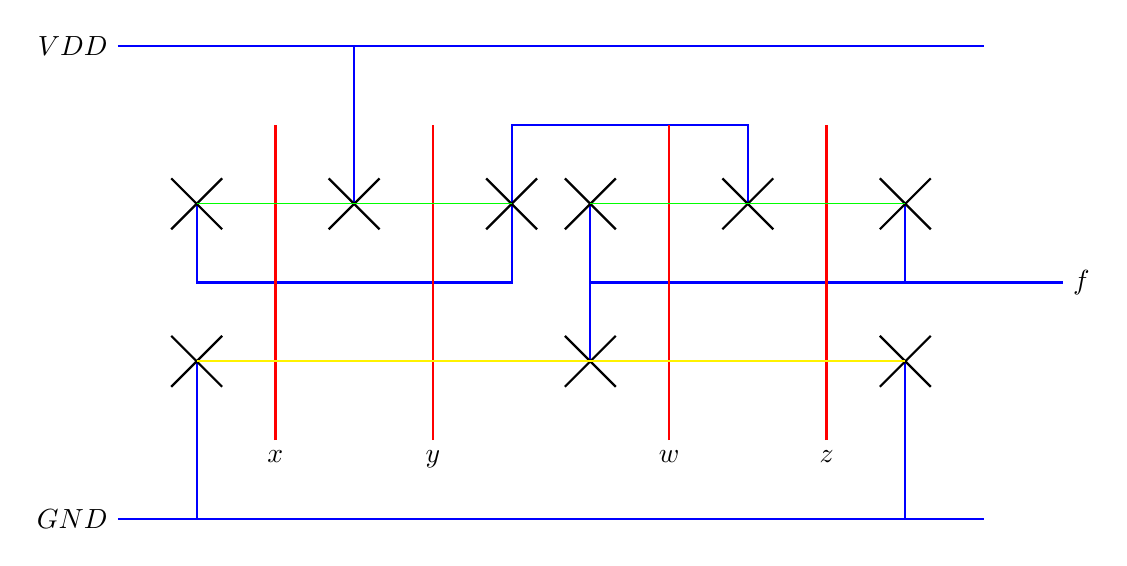
\begin{tikzpicture}
		\draw[blue,thick]
		(0,0) node[left,black] {$GND$} -- (11,0)
		(1,0) -- (1,2) node[cross] {}
		(10,0) -- (10,2) node[cross] {}
		(0,6) node[left,black] {$VDD$} -- (11,6)
		(6,2) node[cross] {} -- (6,4) node[cross] {}
		(6,3) -- (10,3) -- (10,4) node[cross] {}
		(10,3) -- (12,3) node[right,black] {$f$}
		(1,4) node[cross] {} -- (1,3) -- (5,3) -- (5,4) node[cross] {} -- (5,5) -- (8,5) -- (8,4) node[cross] {}
		(3,6) -- (3,4) node[cross] {}
		;

		\draw[red,thick]
		(2,1) node[below,black] {$x$} -- ++ (0,4)
		(4,1) node[below,black] {$y$} -- ++ (0,4)
		(7,1) node[below,black] {$w$} -- ++ (0,4)
		(9,1) node[below,black] {$z$} -- ++ (0,4)
		;

		\draw[yellow,thick]
		(1,2) -- (10,2)
		;

		\draw[yellow,green]
		(1,4) -- (5,4)
		(6,4) -- (10,4)
		;

	\end{tikzpicture}
	\caption{}
	\label{}
\end{figure}

\subsection{Layout}

\subsection{Transition time}

\subsubsection{Size 1}

\begin{figure}[H]
	\centering
	\begin{tikzpicture}
		\begin{axis} [ylabel=$T_{pdr}/s$,xlabel=Transition$/ps$,legend pos=outer north east]
		\addlegendentry{$\mathrm{C}_{inv}$}
		\addplot table [x=Transition,y=tpdr,col sep = tab] {./data/complex/size1/cin1.csv};
		\addlegendentry{$2\mathrm{C}_{inv}$}
		\addplot table [x=Transition,y=tpdr,col sep = tab] {./data/complex/size1/cin2.csv};
		\addlegendentry{$4\mathrm{C}_{inv}$}
		\addplot table [x=Transition,y=tpdr,col sep = tab] {./data/complex/size1/cin4.csv};
		\addlegendentry{$8\mathrm{C}_{inv}$}
		\addplot table [x=Transition,y=tpdr,col sep = tab] {./data/complex/size1/cin8.csv};
		\end{axis}
	\end{tikzpicture}
	\caption{}
	\label{}
\end{figure}

\subsubsection{Size 2}

\begin{figure}[H]
	\centering
	\begin{tikzpicture}
		\begin{axis} [ylabel=$T_{pdr}/s$,xlabel=Transition$/ps$,legend pos=outer north east]
		\addlegendentry{$\mathrm{C}_{inv}$}
		\addplot table [x=Transition,y=tpdr,col sep = tab] {./data/complex/size2/cin1.csv};
		\addlegendentry{$2\mathrm{C}_{inv}$}
		\addplot table [x=Transition,y=tpdr,col sep = tab] {./data/complex/size2/cin2.csv};
		\addlegendentry{$4\mathrm{C}_{inv}$}
		\addplot table [x=Transition,y=tpdr,col sep = tab] {./data/complex/size2/cin4.csv};
		\addlegendentry{$8\mathrm{C}_{inv}$}
		\addplot table [x=Transition,y=tpdr,col sep = tab] {./data/complex/size2/cin8.csv};
		\end{axis}
	\end{tikzpicture}
	\caption{}
	\label{}
\end{figure}

\subsubsection{Size 4}

\begin{figure}[H]
	\centering
	\begin{tikzpicture}
		\begin{axis} [ylabel=$T_{pdr}/s$,xlabel=Transition$/ps$,legend pos=outer north east]
		\addlegendentry{$\mathrm{C}_{inv}$}
		\addplot table [x=Transition,y=tpdr,col sep = tab] {./data/complex/size4/cin1.csv};
		\addlegendentry{$2\mathrm{C}_{inv}$}
		\addplot table [x=Transition,y=tpdr,col sep = tab] {./data/complex/size4/cin2.csv};
		\addlegendentry{$4\mathrm{C}_{inv}$}
		\addplot table [x=Transition,y=tpdr,col sep = tab] {./data/complex/size4/cin4.csv};
		\addlegendentry{$8\mathrm{C}_{inv}$}
		\addplot table [x=Transition,y=tpdr,col sep = tab] {./data/complex/size4/cin8.csv};
		\end{axis}
	\end{tikzpicture}
	\caption{}
	\label{}
\end{figure}

\subsection{Data collection}

\subsection{Minimum cell height}

\end{document}
